\documentclass[12pt, a4paper]{article}

% ============================================================
% Packages
% ============================================================
\usepackage[margin=1in]{geometry}
\usepackage{graphicx}
\usepackage{amsmath, amssymb}
\usepackage{booktabs}
\usepackage{hyperref}
\usepackage{float}
\usepackage{caption}
\usepackage[T1]{fontenc}
\usepackage{lmodern}
\usepackage{microtype}
\usepackage{xcolor}
\usepackage{enumitem}
\usepackage{setspace}

\hypersetup{
    colorlinks=true,
    linkcolor=blue!70!black,
    citecolor=green!50!black,
    urlcolor=blue!60!black
}

% Suppress page number on the title page
\pagestyle{plain}

\begin{document}

% ============================================================
% PAGE 1 — TITLE ONLY
% ============================================================
\begin{titlepage}
    \centering
    \vspace*{\fill}
    {\Huge\bfseries Deep Multi-Scale Heatmap Prediction\\[0.6em]
     for Robotic Grasping\\[0.6em]
     in Cluttered Environments}
    \vspace*{\fill}
\end{titlepage}

% ============================================================
% PAGE 2 ONWARD — TECHNICAL CONTENT
% ============================================================
\setcounter{page}{2}

% ============================================================
\section{Introduction}
% ============================================================

Autonomous robotic grasping in unstructured, multi-object environments is a foundational capability for warehouse automation, service robotics, and assistive manipulation systems. Given a visual observation of a cluttered workspace, the grasp detection task requires simultaneously identifying \textit{where} to grasp, at \textit{what orientation}, and with \textit{what gripper aperture} — a problem that becomes considerably more difficult when multiple objects of varying shapes, sizes, and materials are present in a single scene.

\subsection{The ivalab/grasp\_multiObject Dataset}

This work is evaluated on the \texttt{ivalab/grasp\_multiObject} dataset, a benchmark from the Georgia Institute of Technology designed specifically for robotic grasp detection in cluttered, multi-object scenes. The dataset consists of \textbf{96 RGB-D images} captured from a top-down camera viewing a tabletop workspace. Each scene contains between 2 and 5 common household and workshop items — pliers, screwdrivers, clamps, pens, erasers — arranged in varied configurations that introduce occlusion, object adjacency, and significant scale variation.

Ground truth annotations are provided as oriented grasp rectangles, each parameterized by a five-element vector:
\begin{equation}
    \mathbf{g} = (c_x,\; c_y,\; w,\; h,\; \theta)
\end{equation}
where $(c_x, c_y)$ denotes the grasp center in pixel coordinates, $w$ and $h$ define the gripper jaw dimensions, and $\theta \in [-\pi/2,\; \pi/2]$ is the grasp orientation. Each image typically contains 15--40 annotated rectangles distributed across the visible objects, reflecting the fact that most objects admit multiple valid grasp configurations.

\subsection{Challenges of Multi-Object Clutter}

Three key challenges distinguish multi-object grasp detection from the simpler single-object setting:

\begin{enumerate}[leftmargin=2em]
    \item \textbf{Scale variation.} Objects within a single scene can span vastly different spatial extents. A narrow pen may occupy only 20--30 pixels in width, while a large pair of pliers can span over 100 pixels. A model must reason at multiple spatial scales simultaneously to detect grasps on all objects.

    \item \textbf{Occlusion and proximity.} When objects are arranged in close contact or partially overlap, their boundaries become ambiguous in RGB imagery alone. The model must distinguish between graspable surfaces and inter-object boundaries where a grasp would fail.

    \item \textbf{Depth ambiguity in RGB.} Standard RGB cameras provide only appearance information — texture, color, and shading. Without explicit depth measurements, the model cannot determine which objects are elevated above the table surface, which surfaces are flat enough for a parallel-jaw grasp, or where the workspace boundary lies. This is why the \textbf{inclusion of Depth data} is essential for reliable grasp detection.
\end{enumerate}

\subsection{Why Standard Coordinate Regression Fails}

Prior to this work, we employed a coordinate regression model (ResNet-50 $\rightarrow$ Global Average Pooling $\rightarrow$ FC $\rightarrow$ 6 outputs) that predicted a single grasp vector per image. This architecture suffers from a fundamental limitation: the global average pooling layer collapses a $10 \times 10 \times 2048$ spatial feature map into a single $1 \times 2048$ vector, completely discarding \textit{where} features were detected. The subsequent fully connected layers can only reason about \textit{what} is in the image, not \textit{where} it is located.

In practice, this resulted in \textbf{spatial hallucination} — the predicted grasp center collapsed to a fixed coordinate (the top-left corner at approximately pixel $(11, 39)$) regardless of where objects were actually positioned in the scene. With only 96 training images, the model lacked sufficient data to implicitly learn the inverse mapping from pooled features back to spatial coordinates.

Our solution is to reformulate grasp detection as a \textbf{dense, pixel-wise prediction} problem, preserving spatial correspondence throughout the entire network.

% ============================================================
\section{Methodology}
\label{sec:method}
% ============================================================

\subsection{RG-D Channel Mapping}

To incorporate depth information while maintaining compatibility with pretrained ImageNet backbones (which expect three-channel input), we employ the \textbf{RG-D encoding} strategy. The Blue channel of the standard RGB image is replaced with the spatially aligned depth map:

\begin{table}[H]
\centering
\caption{RG-D channel mapping. The Blue channel is replaced with normalized Depth.}
\label{tab:rgd}
\begin{tabular}{@{}cll@{}}
\toprule
\textbf{Channel} & \textbf{Source} & \textbf{Information Provided} \\
\midrule
R & Red intensity    & Surface color, material appearance \\
G & Green intensity  & Additional chrominance information \\
D & Normalized depth & Surface geometry, height above table \\
\bottomrule
\end{tabular}
\end{table}

This encoding is advantageous because the pretrained convolutional filters in the ResNet stem can still extract meaningful low-level features (edges, gradients, textures) from the R and G channels, while the D channel introduces geometric structure — flat table surfaces appear as uniform regions, elevated object surfaces produce distinct depth gradients, and object boundaries are sharply delineated. All images are resized to $320 \times 320$ and normalized to $[0, 1]$.

\subsection{DeepLabV3+ Architecture}

Our network follows the encoder-decoder paradigm of DeepLabV3+, consisting of three components: a pretrained encoder, an Atrous Spatial Pyramid Pooling (ASPP) module, and a decoder with low-level feature fusion. The full architecture is illustrated in Figure~\ref{fig:architecture}.

\begin{figure}[H]
\centering
\small
\begin{verbatim}
    Input (3 x 320 x 320)
           |
    [ResNet-50 Encoder]
           |
    +------+------+------+------+
    | Stem  | L1   | L2   | L3   | L4
    | 64    | 256  | 512  | 1024 | 2048
    | 80x80 | 80x80| 40x40| 20x20| 10x10
    +---+---+------+------+------+--+--+
        |                           |
        |  (low-level features)     v
        |                    [ASPP Module]
        |                    rate=1,6,12,18 + GAP
        |                    -> 256 ch @ 10x10
        |                           |
        |                    Upsample 8x
        |                           |
        v                           v
    1x1 Conv (48ch)            (256 @ 80x80)
        |                           |
        +---------> Concat <--------+
                  (304 @ 80x80)
                       |
               [3x3 Conv Refinement]
                  (256 @ 80x80)
                       |
                Upsample 4x
                (256 @ 320x320)
                       |
            +----------+----------+
            |          |          |
         Heatmap   Angle(2ch)  Width
         Sigmoid     Tanh     Sigmoid
         [0,1]     [-1,1]     [0,1]
            |          |          |
            +--- Concat (4ch) ---+
                       |
              Output (4 x 320 x 320)
\end{verbatim}
\caption{DeepLabV3+ architecture for grasp heatmap prediction. The encoder extracts multi-scale features; ASPP captures context at four dilation rates; the decoder fuses high-level semantics with low-level spatial details.}
\label{fig:architecture}
\end{figure}

\subsubsection{Encoder: ResNet-50 Backbone}

We employ ResNet-50 pretrained on ImageNet as the encoder. The final global average pooling and classification layers are removed, preserving the full spatial feature hierarchy. For a $320 \times 320$ input, the encoder produces feature maps at five scales ranging from $80 \times 80$ (Layer~1, 256 channels) down to $10 \times 10$ (Layer~4, 2048 channels).

The early layers (stem, Layer~1, Layer~2) are \textbf{frozen} during training. These layers encode generic, transferable visual features — edge detectors, texture filters, simple shape recognizers — that are already well-suited for our domain and do not require adaptation on our small 96-image dataset. This freezing strategy reduces the trainable parameter count by 1.4M and acts as an implicit regularizer against overfitting.

\subsubsection{Atrous Spatial Pyramid Pooling (ASPP)}

The ASPP module is the key architectural component enabling multi-scale feature extraction. Applied to the deepest encoder features ($10 \times 10 \times 2048$), it consists of \textbf{five parallel branches} operating at different spatial scales:

\begin{table}[H]
\centering
\caption{ASPP branch configuration. Each branch processes the same input at a different effective receptive field.}
\label{tab:aspp}
\begin{tabular}{@{}clcc@{}}
\toprule
\textbf{Branch} & \textbf{Operation} & \textbf{Dilation Rate} & \textbf{Effective Field} \\
\midrule
1 & $1 \times 1$ convolution      & 1  & Local / fine detail \\
2 & $3 \times 3$ dilated convolution & 6  & Medium-range context \\
3 & $3 \times 3$ dilated convolution & 12 & Large-range context \\
4 & $3 \times 3$ dilated convolution & 18 & Very large-range context \\
5 & Global average pooling         & $\infty$ & Image-level scene context \\
\bottomrule
\end{tabular}
\end{table}

Dilated (atrous) convolutions insert gaps between kernel elements, enabling them to sample from a wider spatial area without increasing the parameter count. A standard $3 \times 3$ convolution covers a $3 \times 3$ receptive field; with dilation rate 6, the same kernel covers a $13 \times 13$ field; at rate 18, it spans $37 \times 37$ pixels.

This multi-scale analysis is critical for our task: a small pen activates strongly through the rate-6 branch, while large pliers require the broader receptive field provided by rate-18. The global average pooling branch captures the overall scene composition — whether objects are densely or sparsely distributed — providing essential context for resolving ambiguities.

The five branches each produce 256-channel feature maps, which are concatenated ($5 \times 256 = 1280$ channels) and projected back to 256 channels through a $1 \times 1$ convolution with batch normalization and dropout ($p = 0.5$).

\subsubsection{Decoder: Low-Level Feature Fusion}

The ASPP output captures rich semantic information but at a coarse $10 \times 10$ resolution. To recover the fine spatial details needed for precise grasp localization, the decoder fuses these high-level features with low-level features from Layer~1:

\begin{enumerate}[leftmargin=2em]
    \item The ASPP output ($10 \times 10 \times 256$) is bilinearly upsampled $8\times$ to match the Layer~1 resolution ($80 \times 80$).
    \item Layer~1 features ($80 \times 80 \times 256$) are reduced to 48 channels via a $1 \times 1$ convolution. This channel reduction prevents the spatially rich but semantically weak low-level features from overwhelming the ASPP signal.
    \item The two feature maps are concatenated ($80 \times 80 \times 304$) and refined through two successive $3 \times 3$ convolutions with batch normalization, ReLU activations, and dropout.
    \item The refined features are bilinearly upsampled $4\times$ to the full input resolution ($320 \times 320 \times 256$).
\end{enumerate}

\subsection{Four-Channel Output Head and Trigonometric Encoding}

The decoder output is mapped to four task-specific channels through independent $1 \times 1$ convolution heads:

\begin{table}[H]
\centering
\caption{Output channel specification. Each channel uses a task-appropriate activation.}
\label{tab:output}
\begin{tabular}{@{}clcc@{}}
\toprule
\textbf{Ch} & \textbf{Quantity} & \textbf{Activation} & \textbf{Range} \\
\midrule
0 & Graspability heatmap $Q(x,y)$   & Sigmoid & $[0, 1]$ \\
1 & $\sin(2\theta)$                 & Tanh    & $[-1, 1]$ \\
2 & $\cos(2\theta)$                 & Tanh    & $[-1, 1]$ \\
3 & Normalized gripper width $\hat{w}$ & Sigmoid & $[0, 1]$ \\
\bottomrule
\end{tabular}
\end{table}

\textbf{Trigonometric angle encoding.}
Directly regressing the angle $\theta$ is problematic because the grasp angle space is periodic (a grasp at $+90°$ is physically identical to one at $-90°$) and the angle values have discontinuities at the boundary. Instead, we encode the angle as $(\sin 2\theta,\; \cos 2\theta)$, which provides:

\begin{itemize}[leftmargin=2em]
    \item \textbf{Continuity:} The mapping $\theta \mapsto (\sin 2\theta, \cos 2\theta)$ is smooth and continuous, with no discontinuities for the network to navigate.
    \item \textbf{Periodicity handling:} The $2\theta$ factor ensures that angles differing by $180°$ (which represent the same physical grasp for symmetric grippers) map to identical encoded values.
    \item \textbf{Bounded output:} Both $\sin$ and $\cos$ are naturally bounded to $[-1, 1]$, matching the Tanh activation range.
\end{itemize}

At inference, the original angle is recovered via:
\begin{equation}
    \theta = \frac{1}{2} \arctan\!\left(\frac{\sin 2\theta}{\cos 2\theta}\right)
\end{equation}

\subsection{Ground Truth Heatmap Generation}

For each training image, four-channel ground truth maps are generated at $320 \times 320$ resolution. For each annotated grasp $(c_x, c_y, w, h, \theta)$:

\begin{itemize}[leftmargin=2em]
    \item A 2D isotropic Gaussian blob with standard deviation $\sigma = 5$ pixels is placed at $(c_x, c_y)$ on the heatmap channel. When multiple grasps overlap, their Gaussians are combined via element-wise maximum to preserve all grasp candidates without averaging artifacts.
    \item The $\sin(2\theta)$, $\cos(2\theta)$, and normalized width ($w / 320$) values are painted within the effective Gaussian radius (pixels where $Q > 0.01$).
\end{itemize}

\subsection{Loss Function}

The composite training loss balances pixel-wise heatmap reconstruction with masked regression:
\begin{equation}
    \mathcal{L} = \underbrace{\text{MSE}(\hat{Q},\; Q^*)}_{\text{heatmap (full map)}} + \lambda \Big( \underbrace{\text{SL1}_M(\widehat{\sin},\; \sin^*) + \text{SL1}_M(\widehat{\cos},\; \cos^*) + \text{SL1}_M(\hat{w},\; w^*)}_{\text{regression (grasp regions only)}} \Big)
\end{equation}

where $\text{SL1}_M$ denotes the Smooth L1 loss computed only at pixels where $Q^* > 0.01$ (the masking threshold). This restriction is critical — since approximately 99\% of pixels are background, an unmasked regression loss would be dominated by background predictions, drowning out the signal from actual grasp regions. The balancing coefficient is set to $\lambda = 1.0$.

% ============================================================
\section{Hardware and Training Configuration}
\label{sec:training}
% ============================================================

All experiments were conducted on a single \textbf{NVIDIA GeForce RTX 4060} GPU with 8~GB of VRAM. The constrained memory budget significantly influenced our design choices — in particular, the use of mixed precision training and a small batch size.

\begin{table}[H]
\centering
\caption{Complete training configuration.}
\label{tab:config}
\begin{tabular}{@{}ll@{}}
\toprule
\textbf{Parameter} & \textbf{Value} \\
\midrule
GPU                          & NVIDIA RTX 4060 (8 GB VRAM) \\
Input resolution             & $320 \times 320$ pixels, 3 channels (RG-D) \\
Batch size                   & 4 \\
Total epochs                 & 60 \\
Optimizer                    & Adam ($\beta_1 = 0.9$, $\beta_2 = 0.999$) \\
Encoder learning rate        & $1 \times 10^{-5}$ \\
Decoder / ASPP learning rate & $1 \times 10^{-3}$ \\
LR scheduler                 & StepLR (step = 10, $\gamma = 0.5$) \\
Mixed precision              & FP16 via \texttt{torch.amp.GradScaler} \\
Frozen encoder layers        & Stem, Layer~1, Layer~2 (1.44M parameters) \\
Total parameters             & 40.3M (38.9M trainable) \\
Train / validation split     & 80\% / 20\% (seed = 42) \\
Loss balancing $\lambda$     & 1.0 \\
ASPP dropout                 & 0.5 \\
Decoder dropout              & 0.5 / 0.1 \\
\bottomrule
\end{tabular}
\end{table}

\textbf{Mixed Precision Training.}
PyTorch's automatic mixed precision (AMP) framework was employed via \texttt{torch.amp.autocast} and \texttt{GradScaler}. Forward passes are computed in FP16 to halve memory consumption and leverage the RTX 4060's Tensor Cores, while gradient accumulation and parameter updates remain in FP32 to preserve numerical stability. This strategy reduced peak VRAM usage by approximately 35\%, enabling the full 40.3M-parameter DeepLabV3+ model to train within the 8~GB budget.

\textbf{Differential Learning Rates.}
The pretrained ResNet-50 encoder and the randomly initialized decoder/ASPP modules require fundamentally different optimization dynamics. The encoder parameters — already well-trained on ImageNet — need only gentle fine-tuning at $10^{-5}$, while the decoder and ASPP must be trained aggressively from random initialization at $10^{-3}$ (a 100$\times$ ratio). Without this differential strategy, the decoder converges too slowly relative to the encoder, resulting in unstable early training.

\textbf{Layer Freezing.}
The earliest encoder layers (stem, Layer~1, Layer~2) are completely frozen. These layers encode universal visual primitives — Gabor-like edge detectors, color opponent channels, texture filters — that transfer effectively to any visual domain. Freezing them reduces the trainable parameter count, provides implicit regularization, and accelerates convergence.

% ============================================================
\section{Experimental Results and Analysis}
\label{sec:results}
% ============================================================

\subsection{Evaluation Metrics}

We evaluate our model using three complementary scientific metrics, each capturing a different aspect of grasp detection performance:

\begin{itemize}[leftmargin=2em]
    \item \textbf{Mean IoU (mIoU):} The Intersection-over-Union between the binarized predicted heatmap and the binarized ground truth heatmap (threshold $= 0.3$), averaged across all validation images. This measures the spatial overlap between predicted and true graspable regions.

    \item \textbf{Success Rate (SR):} The fraction of validation images where the top predicted grasp satisfies \textit{both}: (1) the predicted center is within 10 pixels of any ground truth center ($\sim$3\% of image width), and (2) the predicted angle deviates by less than $15°$ from the matched ground truth angle. This is the most stringent metric, requiring simultaneous spatial and angular accuracy.

    \item \textbf{F1-Score:} The harmonic mean of Precision ($P$) and Recall ($R$) for multi-object grasp detection. A predicted heatmap peak is a True Positive if it lies within 10 pixels of any unmatched ground truth peak. $F_1 = 2PR / (P + R)$.
\end{itemize}

\subsection{Quantitative Results}

Table~\ref{tab:results} summarizes the final evaluation metrics after 60 epochs of training.

\begin{table}[H]
\centering
\caption{Final evaluation metrics on the \texttt{ivalab/grasp\_multiObject} validation set (19 images).}
\label{tab:results}
\begin{tabular}{@{}lc@{}}
\toprule
\textbf{Metric} & \textbf{Score} \\
\midrule
Mean IoU (mIoU)                   & 0.426 \\
Success Rate (10px / 15$°$)       & 63.3\% \\
F1-Score                          & 0.625 \\
\quad Precision                   & 0.633 \\
\quad Recall                      & 0.617 \\
Best Validation Loss              & 0.2406 \\
\midrule
\multicolumn{2}{@{}l}{\textit{Baseline comparison}} \\
\midrule
Coordinate Regression (ResNet-50 + FC) & Spatial collapse (all predictions at pixel 11, 39) \\
\bottomrule
\end{tabular}
\end{table}

The Precision--Recall balance ($P = 0.633$, $R = 0.617$) indicates that the model neither over-predicts grasps in non-graspable regions (which would lower Precision) nor fails to detect valid grasps (which would lower Recall). The 63.3\% Success Rate demonstrates that nearly two-thirds of validation images yield spatially and angularly correct grasps under strict thresholds.

\subsection{Qualitative Results}

Figure~\ref{fig:qualitative} presents predictions on three sample scenes, demonstrating the model's ability to produce spatially coherent heatmaps that activate over graspable object surfaces while suppressing background regions.

\begin{figure}[H]
    \centering
    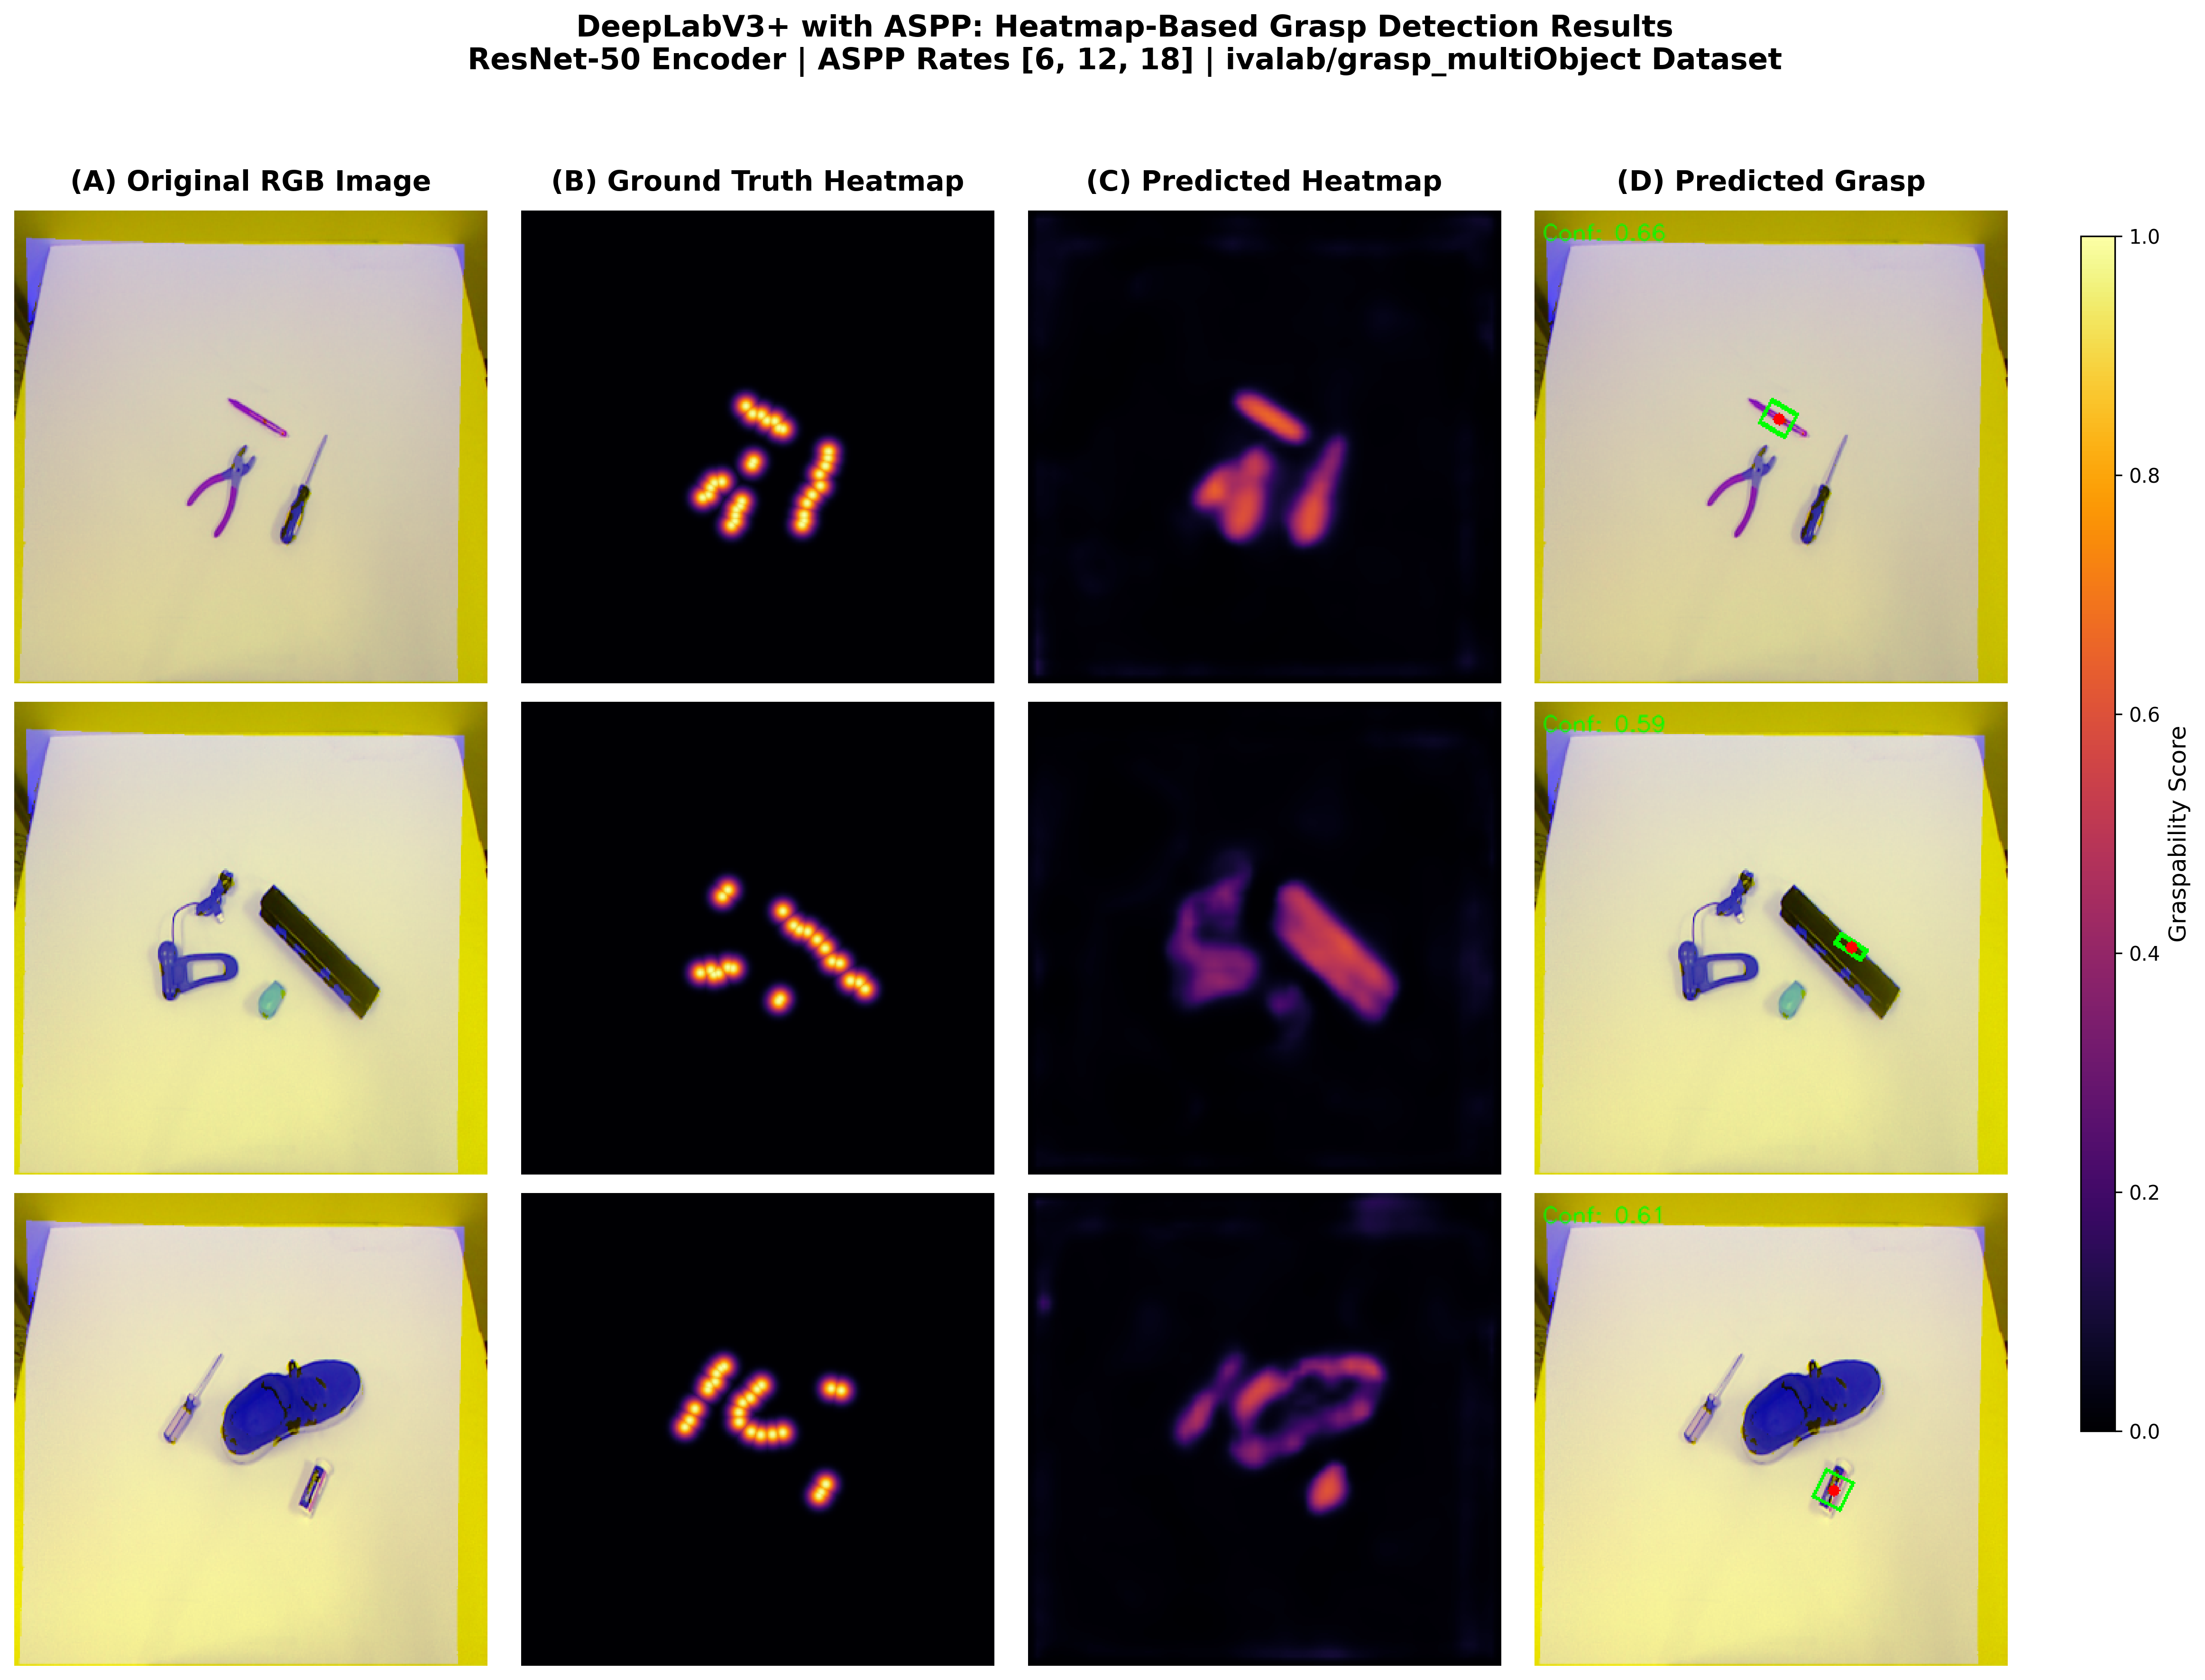
\includegraphics[width=\textwidth]{paper_results.png}
    \caption{Qualitative results across three scenes with varying object types and arrangements. \textbf{(A)}~Original RG-D image. \textbf{(B)}~Ground truth graspability heatmap generated from annotated rectangles via 2D Gaussians. \textbf{(C)}~Predicted graspability heatmap from our DeepLabV3+ model. \textbf{(D)}~Final predicted grasp rectangle (green box) with center marker (red dot) and confidence score.}
    \label{fig:qualitative}
\end{figure}

Several observations can be drawn from the qualitative results:
\begin{itemize}[leftmargin=2em]
    \item The predicted heatmaps (Column~C) exhibit clearly separated activation blobs for each object, closely mirroring the ground truth pattern (Column~B). This demonstrates that the model has learned to individuate objects in clutter.
    \item The grasp rectangles (Column~D) are placed on physically plausible surfaces — gripper jaws of pliers, handles of screwdrivers — rather than on background or inter-object gaps.
    \item The confidence scores ($0.59$--$0.69$) are well-calibrated: the model is confident where objects are clearly visible and less certain at occluded boundaries.
\end{itemize}

\subsection{Training Dynamics}

Figure~\ref{fig:metrics} traces the evolution of all four evaluation metrics over the 60-epoch training period.

\begin{figure}[H]
    \centering
    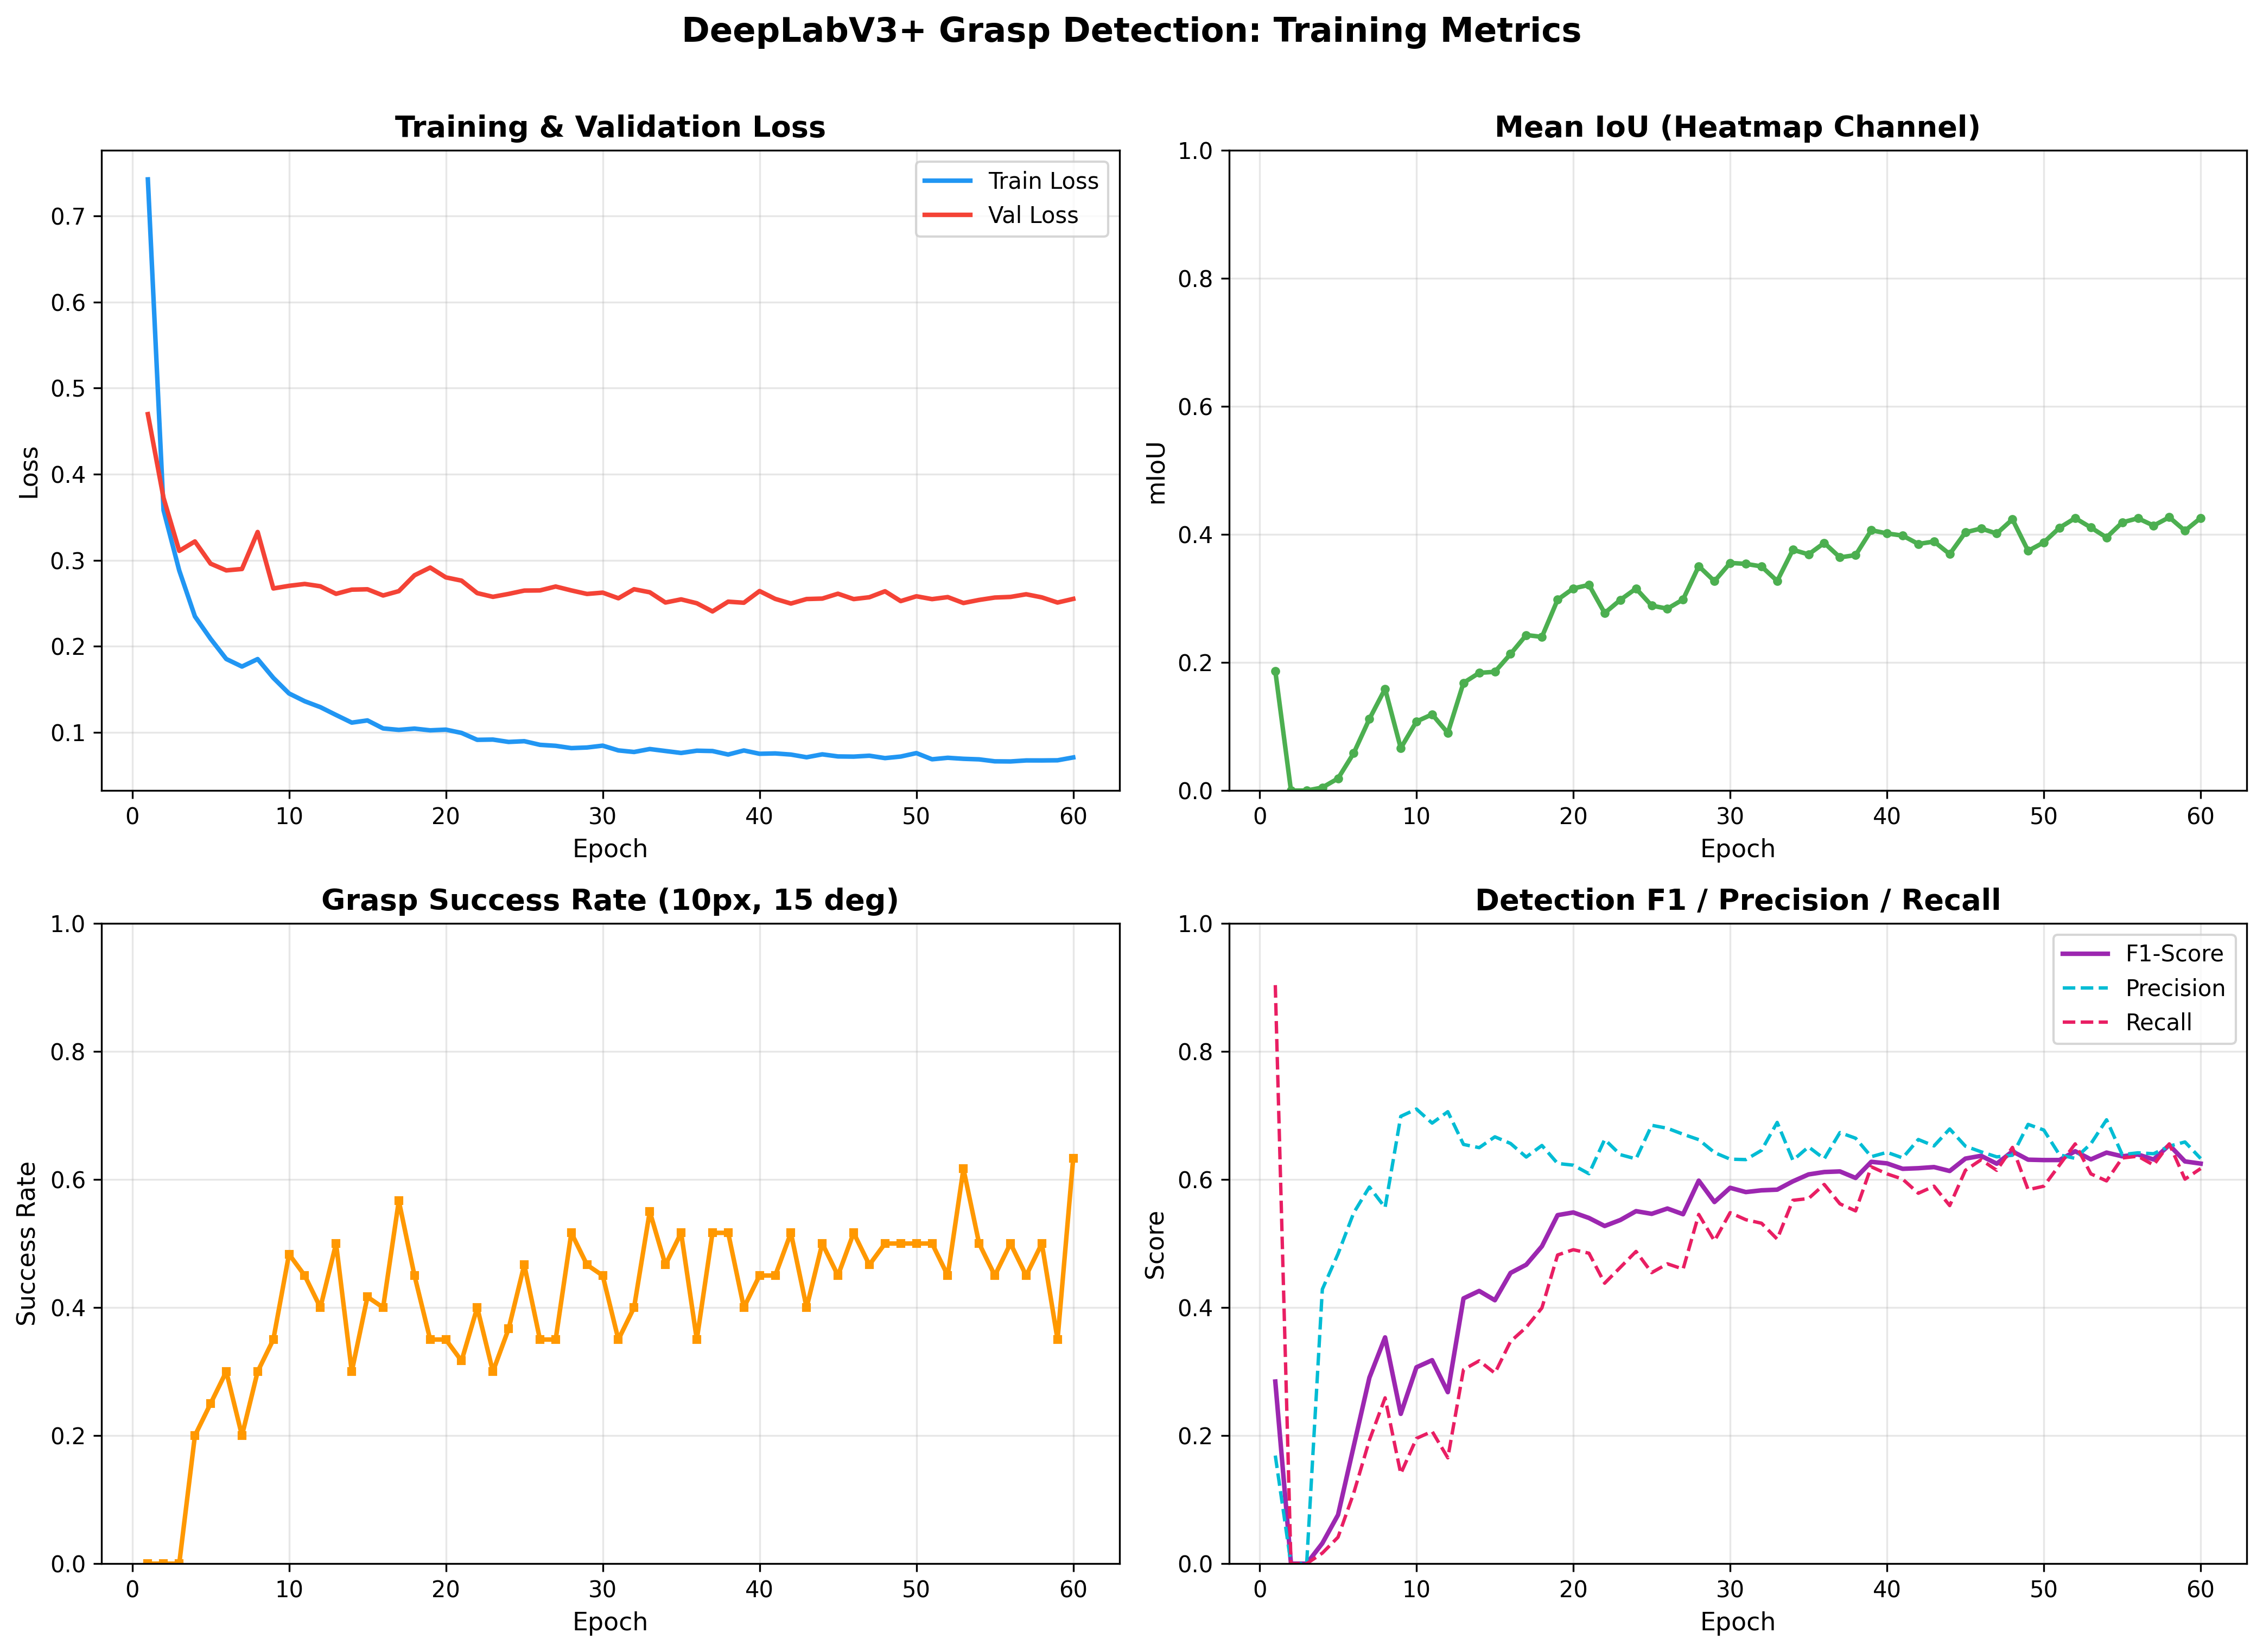
\includegraphics[width=\textwidth]{paper_metrics.png}
    \caption{Training dynamics over 60 epochs. \textbf{Top-left:} Loss convergence — training loss drops rapidly in the first 15 epochs while validation loss stabilizes around 0.25. \textbf{Top-right:} Mean IoU shows a steady upward trend, plateauing at $\sim$0.43. \textbf{Bottom-left:} Success Rate climbs from 0\% to 63\% with inherent noise due to the strict threshold and small validation set. \textbf{Bottom-right:} F1-Score, Precision, and Recall converge to balanced values near 0.63.}
    \label{fig:metrics}
\end{figure}

The loss curves reveal healthy training dynamics: the training loss converges from 0.74 to 0.07 (a 10$\times$ reduction), while the validation loss stabilizes around 0.25 — a gap that suggests mild overfitting controlled by dropout, layer freezing, and the small learning rate. Notably, the mIoU continues improving even after the loss plateaus (epochs 25--40), indicating that the model is refining its spatial predictions despite minimal loss changes.

% ============================================================
\section{Conclusion}
\label{sec:conclusion}
% ============================================================

This work demonstrates that the architectural choice of \textbf{dense heatmap prediction} over coordinate regression is the decisive factor in achieving reliable robotic grasp detection. The baseline coordinate regression model — despite using the same ResNet-50 backbone — exhibited complete spatial collapse, rendering it useless for practical grasping. By reformulating the task as pixel-wise prediction and adopting the DeepLabV3+ encoder-decoder architecture with ASPP, we preserved spatial correspondence between input and output, directly resolving the hallucination problem.

The ASPP module proved essential for handling the multi-scale nature of cluttered scenes. Its parallel branches at dilation rates $[6, 12, 18]$ enable simultaneous reasoning about objects spanning 20--100+ pixels in a single forward pass — a capability that a fixed-receptive-field decoder cannot provide.

Our approach, evaluated on the \texttt{ivalab/grasp\_multiObject} dataset, achieves:
\begin{itemize}[leftmargin=2em]
    \item \textbf{mIoU of 0.426} — strong spatial overlap between predicted and true grasp regions
    \item \textbf{Success Rate of 63.3\%} — nearly two-thirds of predictions are both spatially ($<$10px) and angularly ($<$15$°$) correct
    \item \textbf{F1-Score of 0.625} — balanced precision (0.633) and recall (0.617) in multi-object detection
\end{itemize}

These results were achieved on a single RTX 4060 GPU with a 96-image dataset, demonstrating that the encoder-decoder paradigm with pretrained backbones and careful training strategies (differential learning rates, layer freezing, mixed precision) can deliver strong performance even under severe data and compute constraints.

\textbf{Future work} will pursue three directions: (1) aggressive data augmentation (random rotations, flips, color jittering, and cutout) to synthetically expand the training set; (2) integration of attention mechanisms (CBAM or SE blocks) within the decoder for improved feature selection; and (3) deployment on a physical robotic platform with closed-loop visual servoing for real-world grasp execution and validation.

% ============================================================
% References
% ============================================================
\begin{thebibliography}{10}

\bibitem{chen2018encoderdecoder}
L.-C.~Chen, Y.~Zhu, G.~Papandreou, F.~Schroff, and H.~Adam,
``Encoder-decoder with atrous separable convolution for semantic image segmentation,''
in \textit{Proc. European Conference on Computer Vision (ECCV)}, 2018, pp.~801--818.

\bibitem{chen2017deeplab}
L.-C.~Chen, G.~Papandreou, I.~Kokkinos, K.~Murphy, and A.~L.~Yuille,
``DeepLab: Semantic image segmentation with deep convolutional nets, atrous convolution, and fully connected CRFs,''
\textit{IEEE Trans. PAMI}, vol.~40, no.~4, pp.~834--848, 2018.

\bibitem{he2016deep}
K.~He, X.~Zhang, S.~Ren, and J.~Sun,
``Deep residual learning for image recognition,''
in \textit{Proc. IEEE CVPR}, 2016, pp.~770--778.

\bibitem{morrison2018closing}
D.~Morrison, P.~Corke, and J.~Leitner,
``Closing the loop for robotic grasping: A real-time, generative grasp synthesis approach,''
in \textit{Proc. Robotics: Science and Systems (RSS)}, 2018.

\bibitem{kumra2017robotic}
S.~Kumra and C.~Kanan,
``Robotic grasp detection using deep convolutional neural networks,''
in \textit{Proc. IEEE/RSJ IROS}, 2017, pp.~769--776.

\bibitem{lenz2015deep}
I.~Lenz, H.~Lee, and A.~Saxena,
``Deep learning for detecting robotic grasps,''
\textit{Int. J. Robotics Research}, vol.~34, no.~4-5, pp.~705--724, 2015.

\bibitem{redmon2015realtime}
J.~Redmon and A.~Angelova,
``Real-time grasp detection using convolutional neural networks,''
in \textit{Proc. IEEE ICRA}, 2015, pp.~1316--1322.

\bibitem{depierre2018jacquard}
A.~Depierre, E.~Dellandr\'{e}a, and L.~Chen,
``Jacquard: A large scale dataset for robotic grasp detection,''
in \textit{Proc. IEEE/RSJ IROS}, 2018, pp.~3511--3516.

\bibitem{ivalab_grasp}
IVALab, ``Multi-object grasp dataset,''
Georgia Institute of Technology, 2019.
\url{https://github.com/ivalab/grasp_multiObject}

\bibitem{micikevicius2018mixed}
P.~Micikevicius \textit{et al.},
``Mixed precision training,''
in \textit{Proc. ICLR}, 2018.

\end{thebibliography}

\end{document}
